يعرف فضاء عمل أي نظام روبوتي بمجموعة النقاط التي يستطيع الروبوت التواجد فيها بشكل آمن. نذكر هنا أن فضاء العمل لا يكون بالضرورة معرف بأساس الاحداثيات المكانية، على سبيل المثال، يمكن تعريف فضاء عمل ذراع روبوت بدلالة قيم مفاصل هذه الذراع، ويكون عدد أبعاده بعدد درجات حرية الذراع. يستخدم فضاء العمل بشكل أساسي للبحث عن مسارات يستطيع الروبوت عبورها بغية انجاز عمل معين. قد يكون هذا العمل غير مقيد، كإيجاد مسار بين موضع الروبوت الحالي ونقطة هدف محددة مسبقاً، وقد يكون مقيد بشروط معينة كإيجاد أقصر مسار أو أقلها استهلاكاً للطاقة. يمكّننا التعريف الجيد لفضاء العمل من إيجاد قيود المسألة التي يحاول الروبوت حلها بغية إيجاز المهمة الموكلة له، بمعنى أكثر دقة، تشكيل فضاء العمل هو أول خطوة من حل مسألة تخطيط المسار، التي تعتبر مسألة أمثلة.
يبين الشكل \ref{15:fig:4} فضاء عمل سرب الروبوتات. يتكون من مربع بضلع 2.4 متر وحواف مرتفعة. يحتوي المربع على عدة عوائق بأشكال مكعب أو أسطوانة وبأبعاد مختلفة. يمكن للعوائق أن تتحرك بالشكل المطلوب على الشبكة لتشكيل فضاء عمل ديناميكي.
 
 \begin{figure}[h]
 	\centering
 	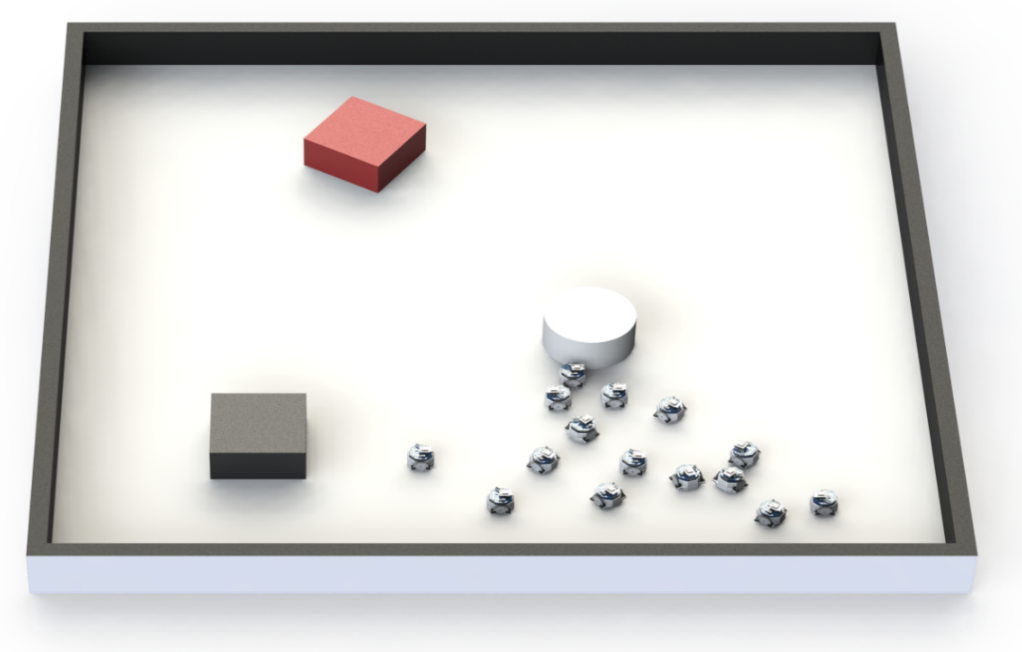
\includegraphics[width=0.8\linewidth]{figs/15/fig4}
 	\caption{ إخراج ثلاثي الأبعاد لمنصة العمل}
 	\label{15:fig:4}
 \end{figure}